%!TEX root = ../main.tex

%=============================================================================== 
%
%    Chapter: vectors
%
%=============================================================================== 

\chapter{Vectors}
\label{chapter:vectors}

In this chapter we'll learn how to manipulate multi-dimensional objects called vectors.						\index{vector|textbf}
Vectors are the precise way to describe directions in space.
We need vectors in order to describe physical quantities like forces, velocities, and accelerations.

Vectors are built from ordinary numbers,
which form the \emph{components} of the vector.
You can think of a vector as a list of numbers,
and \emph{vector algebra} as operations
performed on the numbers in the list.
Vectors can also be manipulated as geometric objects,
represented by arrows in space.
For instance, the arrow that corresponds to the vector $\vec{v}=(v_x,v_y)$ starts at the origin $(0,0)$
and ends at the point $(v_x,v_y)$.
The word vector comes from the Latin \emph{vehere},
which means \emph{to carry}.
Indeed, the vector $\vec{v}$ takes the point $(0,0)$ and carries it to the point $(v_x,v_y)$.

\begin{figure}[H]
	\centering
	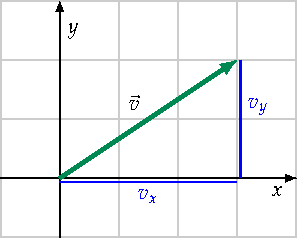
\includegraphics[width=0.4\textwidth]{figures/vectors/vector_components.pdf}
	\vspace{-2mm}
	\caption{	The vector $\vec{v}=(3,2)$ is an arrow in the Cartesian plane.
			The horizontal component of $\vec{v}$ is $v_x=3$
			and the vertical component  is $v_y=2$.}
	\label{fig:vector_components}
\end{figure}




%!TEX root = ../main.tex

%=======================================================================  vectors
\section{Vectors}
\label{sec:vectors}

	Vectors are extremely useful in all areas of life.
	In physics, for example, we use a vector to describe the velocity of an object.
	It is not sufficient to say that the speed of a tennis ball is 200 kilometres per hour:
	we must also specify the direction in which the ball is moving.
	Both of the two velocities 
	\[
	 \vec{v}_1 = (200,0) 
	 \qquad \textrm{and}
	 \qquad \vec{v}_2=(0,200)
	\]
	describe motion at the speed of $200$ kilometres per hour;
	but since one velocity points along the $x$-axis, and the other points along the $y$-axis,
	they are \emph{completely} different velocities. 
	The velocity vector contains information about the object's speed \emph{and} its direction.
	The direction makes a big difference.
	If it turns out the tennis ball is hurtling toward you, you'd better get out of the way!

	The main idea in this chapter is that \textbf{vectors are not the same as numbers}.
	We'll start by defining what vectors are.
	Then we'll describe all the mathematical operations we can perform with vectors,
	which include
		vector addition $\vec{u}+\vec{v}$, 
		vector subtraction $\vec{u}-\vec{v}$,
		vector scaling $\alpha\vec{v}$,
		and other operations.


	\subsection{Definitions}
	\label{vectors:definitions}

		A two-dimensional vector $\vec{v}$ corresponds to a \emph{pair of numbers}:
		\[
			\vec{v} = (v_x, v_y),
		\]
		where $v_x$ is the \emph{$x$-component} of the vector and $v_y$ is its \emph{$y$-component}.					\index{components}
		We denote the set of two-dimensional vectors as $\mathbb{R}^2$,
		since the components of a two-dimensional vector are specified by two real numbers.
		We'll use the mathematical shorthand $\vec{v} \in \mathbb{R}^2$ to define a two-dimensional vector $\vec{v}$.
		Vectors in $\mathbb{R}^2$ can be represented as arrows in the Cartesian plane.
		See the vector $\vec{v}=(3,2)$ illustrated in Figure~\ref{fig:vector_components}.

		We can also define three-dimensional vectors like the vector $\vec{v} = (v_x, v_y, v_z) \in \mathbb{R}^3$,
		which has three components.
		A three-dimensional coordinate system is similar to the Cartesian coordinate system you're familiar with,
		and includes the additional $z$-axis that measures the height above the plane.
		In fact,
		there's no limit to the number of dimensions for vectors.
		We can define vectors in an $n$-dimensional space:								\index{dimension}
		$\vec{v} = (v_1, v_2, \ldots, v_n) \in \mathbb{R}^n$.
		For the sake of simplicity,
		we'll define all the vector operation formulas using two-dimensional vectors.
		Unless otherwise indicated in the text,
		all the formulas we give for two-dimensional vectors $\vec{v} \in \mathbb{R}^2$
		also apply to $n$-dimensional vectors $\vec{v} \in \mathbb{R}^n$.


		\subsubsection{Vector operations}

			Consider two vectors,
			$\vec{u}=(u_x,u_y) $ and $\vec{v}=(v_x,v_y)$,
			and assume that $\alpha \in \mathbb{R}$ is an arbitrary constant. 
			The following operations are defined for these vectors:
			\begin{itemize}
				\item 	\textbf{Addition:}	$\vec{u} + \vec{v} = (u_x+v_x,\, u_y+v_y)$
				\item 	\textbf{Subtraction:}	$\vec{u} - \vec{v} = (u_x-v_x,\, u_y-v_y)$
				\item 	\textbf{Scaling:}		$\alpha \vec{u} = (\alpha u_x,\, \alpha u_y)$
				\item 	\textbf{Dot product:}	$\vec{u} \cdot \vec{v}  = u_xv_x+u_yv_y$								\index{dot product}
				\item 	\textbf{Length:}		$\|\vec{u}\| = \sqrt{\vec{u}\cdot\vec{u}} = \sqrt{u_x^2+u_y^2}$.
						The vector's length is also called the \emph{norm} of the vector.
						We sometimes use the letter $u$ to denote the length of the vector $\vec{u}$.
			\end{itemize}

			\noindent
			Note there is no vector division operation.

			For vectors in a three-dimensional space $\vec{u}=(u_x,u_y,u_z) \in \mathbb{R}^3$
			and $\vec{v}=(v_x,v_y,v_z) \in \mathbb{R}^3$,
			we can also define the \textbf{cross product} operation												\index{cross product}
			$\vec{u} \times \vec{v} = (u_yv_z-u_zv_y,\; u_zv_x-u_xv_z,\; u_xv_y-u_yv_x)$.
			The dot product and the cross product are new operations that you probably haven't seen before.


		\subsubsection{Vector representations}

			We'll use three equivalent ways to denote vectors in two dimensions:
			\begin{itemize}
			    \item   	$\vec{v} =(v_x, v_y)$: component notation.
					The vector is written as a pair of numbers called the \emph{components} or \emph{coordinates} of the vector.	\index{coordinates}
			    \item 	$\vec{v} =v_x\hat{\imath}+ v_y\hat{\jmath}$: unit vector notation.
					The vector is expressed as a combination of the unit vectors
					$\hat{\imath} = (1,0)$ and $ \hat{\jmath} = (0,1)$.
			    \item   	$\vec{v}=\|\vec{v}\|\angle \theta$: length-and-direction notation (polar coordinates).
					The vector is expressed in terms of its \emph{length} $\|\vec{v}\|$
					and the angle $\theta$ that the vector makes with the $x$-axis.
			\end{itemize}

			\begin{figure}[htb]
				\centering
				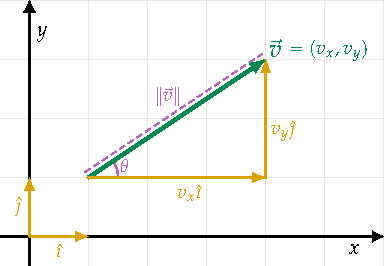
\includegraphics[width=0.6\textwidth]{figures/vectors/vector_components_annotated.pdf}
				\vspace{-2mm}
				\caption{The vector $\vec{v}=(v_x,v_y) = v_x\hat{\imath}+ v_y\hat{\jmath} = \|\vec{v}\|\angle \theta$.}
				\label{fig:vector_components_annotated}
			\end{figure}

			\noindent
			We use the component notation for doing vector algebra calculations since it is most compact.
			The unit vector notation shows explicitly that the vector $\vec{v}$ corresponds to the sum of
			$v_x\hat{\imath}$ (a displacement of $v_x$ steps in the direction of the $x$-axis)
			and $v_y\hat{\jmath}$ (a displacement of $v_y$ steps in the direction of the $y$-axis).
			The length-and-direction notation describes the vector $\vec{v}$
			as a displacement of $\|\vec{v}\|$ steps in the direction of the angle $\theta$.
			We'll use all three ways of denoting vectors throughout the rest of the book,
			and we'll learn how to convert between them.


	\subsection{Exercises}
	\label{basis:exercises}

		%!TEX root = ../main.tex

\begin{exercises}{ch3}

	\begin{exercise}
		Given the vectors $\vec{v}_1=(2,1)$, $\vec{v}_2=(2,-1)$, and $\vec{v}_3=(3,3)$,
		calculate the following expressions:
		\threecol
			\textbf{a)}~$\vec{v}_1 + \vec{v}_2$
			
			\textbf{b)}~$\vec{v}_2 - 2\vec{v}_1$
			
			\textbf{c)}~$\vec{v}_1 + \vec{v}_2 + \vec{v}_3$
		\endthreecol
		
		\begin{eanswer}\textbf{a)}~$(4,0)$.
					\textbf{b)}~$(-2,-3)$.
					\textbf{c)}~$(7,3)$.\end{eanswer}
	\end{exercise}

	\begin{exercise}	\label{exercise:vector-polar-to-cartesian-conversion}
		Express the following vectors as components:
		\threecol
			\textbf{a)}~$\vec{v}_1 =10\angle30^\circ$
			
			\textbf{b)}~$\vec{v}_2 = 12\angle\!-\!90^\circ$
			
			\textbf{c)}~$\vec{v}_3 = 3\angle170^\circ$
		\endthreecol

		\begin{eanswer}\textbf{a)}~$\vec{v}_1=(5\sqrt{3},5)=(8.66,5)$.
					\textbf{b)}~$\vec{v}_2=(0,-12)$.
					\textbf{c)}~$\vec{v}_3=(-2.95,0.52)$.\end{eanswer}
	\end{exercise}


	\begin{exercise}	\label{exercise:vector-cartesian-to-polar-conversion}
		Express the following vectors in length-and-direction notation:
		\threecol
			\textbf{a)}~$\vec{u}_1 = (4,0)$
			
			\textbf{b)}~$\vec{u}_2 = (1,1)$
			
			\textbf{c)}~$\vec{u}_3 = (-1,3)$
		\endthreecol

		\begin{eanswer}\textbf{a)}~$\vec{u}_1=4\angle 0^\circ$. 
					\textbf{b)}~$\vec{u}_2=\sqrt{2}\angle 45^\circ$.
					\textbf{c)}~$\vec{u}_3=\sqrt{10}\angle108.43^\circ$.\end{eanswer}
	\end{exercise}



%		Express the following vectors in terms of unit vectors $\hat{\imath}$, $\hat{\jmath}$, and $\hat{k}$:		%		\threecol
%			
%			
%		\endthreecol
%		\begin{eanswer}\textbf{a)}~$\vec{w}_1=9.06\hat{\imath}  + 4.23\hat{\jmath}$.
%					\textbf{c)}~$\vec{w}_3=7\hat{\imath}  +6 \hat{\jmath} + 5\hat{k}$.\end{eanswer}




\end{exercises}


%!TEX root = ../main.tex

\section{Vectors problems}
\label{sec:vec_problems}

\vspace{-2mm}

You learned a bunch of vector formulas and you saw some vector diagrams,
but did you really learn how to solve problems with vectors?
There is only one way to find out: test yourself by solving problems.

I've said it before and I don't want to repeat myself too much,
but it's worth saying again: the more problems you solve, the better you'll understand the material.
It's now time for you to try the following vector problems to make sure you're on top of things.

\medskip

{ \small

\begin{problems}{ch3}

	\begin{problem}
		Given the vectors $\vec{u}=(1,1,1)$, $\vec{v} = (2,3,1)$, and $\vec{w}=(-1,-1,2)$,
		compute the following products:
		
		\threecol
			\textbf{a)}~$\vec{u} \cdot \vec{v}$

			\textbf{b)}~$\vec{u} \cdot \vec{w}$
			
			\textbf{c)}~$\vec{v} \cdot \vec{w}$
		\endthreecol
		
		\threecol
			\textbf{d)}~$\vec{u} \times \vec{v}$

			\textbf{e)}~$\vec{u} \times \vec{w}$
			
			\textbf{f)}~$\vec{v} \times \vec{w}$
		\endthreecol
		
		\begin{answer}\textbf{a)}~$6$.
					\textbf{b)}~$0$.
					\textbf{c)}~$-3$.
					\textbf{d)}~$(-2, 1, 1)$.
					\textbf{e)}~$(3, -3, 0)$.
					\textbf{f)}~$(7, -5, 1)$.\end{answer}
	\end{problem}


	\begin{problem}
		Given the vectors $\vec{p} =(1,1,0,3,3)$ and $\vec{q}=(1,2,3,4,5)$, calculate the following expressions:
		\threecol
			\textbf{a)}~$\vec{p}+\vec{q}$
			
			\textbf{b)}~$\vec{p}-\vec{q}$
			
			\textbf{c)}~$\vec{p} \cdot \vec{q}$
		\endthreecol
		
		\begin{answer}\textbf{a)}~$(2,3,3,7,8)$.
					\textbf{b)}~$(0,-1,-3,-1,-2)$.
					\textbf{c)}~$30$.\end{answer}
	\end{problem}


	\begin{problem}
		Find a unit vector that is perpendicular to both  $\vec{u}=(1, 0, 1)$ and $\vec{v} =(1, 2, 0)$.
		\begin{hint}
			Use the cross product.
		\end{hint}
		\begin{answer}$(-\frac{2}{3}, \frac{1}{3}, \frac{2}{3})$ or $(\frac{2}{3}, -\frac{1}{3}, -\frac{2}{3})$.\end{answer}
		\begin{solution}See \href{http://bit.ly/1cOa8yo}{\texttt{bit.ly/1cOa8yo}} for calculations.
		\end{solution}
	\end{problem}

	\begin{problem}
		Find a vector that is orthogonal to both $\vec{u}_1 = (1, 0, 1)$ and $\vec{u}_2 =(1, 3, 0)$, 
		 and whose dot product with the vector  $\vec{v}= (1, 1, 0)$ is equal to $8$.
		%	\begin{hint}
		%	\end{hint}
		\begin{answer}$(12, -4, -12)$.\end{answer}
		\begin{solution}
			Any multiple of the vector $\vec{u}_1 \times \vec{u}_2 = (-3,1,3)$ 
			is perpendicular to both $\vec{u}_1$ and 	$\vec{u}_2$.
			We must find a multiplier $t \in \mathbb{R}$ such that 
			$t(-3,1,3) \cdot (1, 1, 0) = 8$.
			Computing the dot product we find $-3t + t = 8$, so $t=-4$.
			The vector we're looking for is $(12, -4, -12)$.
			See \href{http://bit.ly/1nmYH8T}{\texttt{bit.ly/1nmYH8T}} for calculations.
		\end{solution}
	\end{problem}


\end{problems}

} % /small

